\section{Codereview-Systeme, die Git unterstützen}
\label{sec:CRS-Git}

Weil das \ac{CRS} Git unterstützen muss, kommen nur einige in Frage. Hier werden einige davon vorgestellt. Bitbucket in \cref{Bitbucket}, Cruicuble in \cref{subsec:Crucible}, Helix TeamHub in \cref{subsec:HelixTeamHub}, Gerrit in \cref{subsec:Gerrit}, RhodeCode in \cref{subsec:RhodeCode}, Github in \cref{subsec:Github}.

\subsection{Bitbucket}
\label{subsec:Bitbucket}

Bitbucket\footnote{\url{https://bitbucket.org/}} ist ein Quellcode-Management-System, das das \ac{VCS} Git unterstützt. Bitbucket unterstützte nach seinem Entwurf als \ac{VCS} nur Mercurial. 3 Jahren später wurde es um die Unterstützung von Git erweitert. Am 1. Juni 2020 wurde die Unterstützung von Mercurial vollständig eingestellt.

\begin{itemize}
	\item \textbf{Art des Reviews}: \textit{pre- and post-commit} Und die erfolgt durch eine Pull Request
	\item \textbf{Entwickler}: Bitbucket wurde 2007 vom Jesper Nøhr entwickelt und 2010 von Atlassian
		 gekauft.
	\item \textbf{Reviews Workflow}: Erfolgt durch ein Pull Request, was in verschiedenen Abläufen erstellt werden kann z.B.:
		\begin{itemize}
			\item Feature Branch Workflow: Erklärung im \cref{sec:Git-Workflows}
			\item Git flow Workflow: Erklärung im \cref{sec:Git-Workflows}
		\end{itemize}
\end{itemize}

Die \cref{fig:Forking-workflow} verdeutlicht den Feature Branch Workflow.

\begin{description}
	\item [Bitbuckets Vorteile:] \hfill
	\begin{itemize}
		\item Unbegrenzte Anzahl von private Repositories.
		\item Hosting in Cloud oder auf eigenem Server.
		\item \ac{CI}/\ac{CD} sind in Bitbucket integriert.
		\item Erstellen von einer Merge-Checkliste mit zugeordneten Genehmigern.
		\item Für kleine Teams bis 5 Personen bestehen keine Kosten für das Hosten auf Bitbuckets Server.
	\end{itemize}
	
	\item [Bitbuckets Nachteile:] \hfill
	\begin{itemize}
		\item Es besteht keine Möglichkeit, um bestehende gemergte commits zu reviewen.
		\item Das Review ist nur vor dem Zusammenführen von einem Feature-Branch mit dem Master-Branch Möglich.
		\item Um zu hosten auf Bitbucketsever steht für mehr als 5 Personen einen monatlichen Beitrag und für Self-hosten (auf eigenem Server) besteht eine einmalige Zahlung. Der 
			Preis für beide Varianten variiert je nach Personenanzahl.
	\end{itemize}
\end{description}

\subsection{Crucible}
\label{subsec:Crucible}

Crucible ist eine webbasierte Plattform, die ein formelles Codereview anbietet. Sie unterstützt die \acp{VCS} \ac{SVN}, Git, Mercurial, perforce.

\begin{itemize}
	\item \textbf{Art des Reviews}: \textit{pre- and post-commit}
	\item \textbf{Entwickler}: Crucible ist ein Atlassian Produkt
	\item \textbf{Workflow}: Es gibt verschiedene Weisen, wie man einen Review in Crucible durchführen kann. Allerdings werden sich diese nach der an dem Review beteiligten Personen
		 unterscheiden, diese sind:
		\begin{itemize}
			\item Der Moderator. Er ist die Person, die das Review startet und für das Schließen des Reviews verantwortlich ist
			\item Die Reviewer
			\item Der Autor
		\end{itemize}
		Beispiele:
		
		\begin{enumerate}
			\item One-to-One Reviews: Der Autor startet das Review \footnote{Der Autor ist also in diesem Workflow der Moderator}, danach kommentiert der Reviewer und der Autor kann auf diese
				Kommentar reagieren. Das kann sich mehrmals wiederholen bis das Review fertig ist und der Autor diese schließt\\
				Die \cref{fig:one-to-one-workflow} beschreibt diesen Workflow
				\begin{figure}[H]
					\centering
					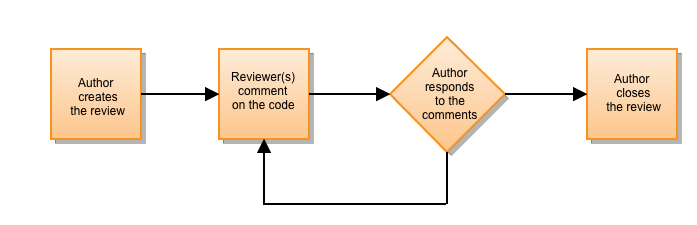
\includegraphics[width=1.0\textwidth]{one-to-one-review}
					\caption[Crucible: one-to-one-review]{Crucible Ablaufsmöglichkeit,\\ \cite{Crucible}}
					\label{fig:one-to-one-workflow}
				\end{figure}
				
			\item Formal group reviews: Der Autor startet das Review und lädt die Reviewer ein. So können die Reviewer diese diskutieren und dementsprechend bekommen die Reviewer 
				die Antworten vom Autor (Der Autor ist in dem Fall auch der Moderator). Jeder Diskussionspunkt wird vom Moderator festgelegt. So bald das Review zu Ende kommt,
				fasst der Moderator das Review zusammen und schließt es\\
				Die \cref{fig:Formal-group-review} zeigt diesen Ablauf
				\begin{figure}[H]
					\centering
					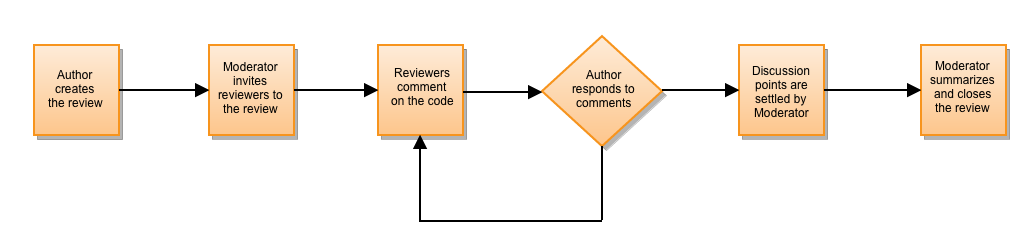
\includegraphics[width=1.0\textwidth]{Formal-group-reviews}
					\caption[Crucible: Formal group review]{Crucible Ablaufsmöglichkeit,\\ \cite{Crucible}}
					\label{fig:Formal-group-review}
				\end{figure}
		\end{enumerate}
		
\end{itemize}

\begin{description}
	\item [Crucibles Vorteile:] \hfill
	\begin{itemize}
		\item Das Review des Inhalts ist flexibel.
		\item Diskussionsrunden um in Bestimmten Quelltextzeilen oder ein bestimmtes Commit sowie einen gesamten Änderungssatz zu Kommentieren.
		\item Nachverfolgen, Maßnahmen ergreifen in Bezug auf das, was der Autor wichtig findet.
		\item Ansicht vom Reviewstatus und wer möglicherweise Überprüfungen aufhält.
		\item Berichte über Stellen im Quelltext, die noch nicht überprüft wurden.
		\item Unterstützt nicht nur Git sonder unterstützt auch \ac{SVN}.
	\end{itemize}
	
	\item [Crucibles Nachteile:] \hfill
	\begin{itemize}
		\item Das Review muss manuell in Git eingefügt werden. D.h. Automatisches Zusammenführen ist nicht möglich.
		\item Schwer zu erzwingen.
	\end{itemize}
\end{description}

\subsection{Helix TeamHub}
\label{subsec:HelixTeamHub}

Helix TeamHub ist eine webbasierte Plattform, die Hosten und Management von Repositories ermöglicht. Sie unterstützt Mercurial, Git, \ac{SVN}, Ivy, und mehr.

\begin{itemize}
	\item \textbf{Art des Reviews}: \textit{pre- and post-commit}
	\item \textbf{Entwickler}: Perforce
	\item \textbf{Reviews Workflow}: Das Review kann in Helix Teamhub eingerichtet werden, so kann das Mitglied, das das Review erstellte, entscheiden, wer die Reviewer
		 sind und welche Änderungen in welchem Branch überprüft werden sollen.
		 Ein Beispiel für einen möglichen Workflow:
		 
		  Git-Feature-Branch-Workfow: Der Ablauf ähnelt sich dem Feature-Branch Workflow von Bitbucket im \cref{subsec:Bitbucket}.
		  Es wird zuerst ein Projekt erstellt und zu diesem Projekt wird ein Repository hinzugefügt. Durch Git wird ein Branch in diesem Repository
		  erstellt. Der Entwickler arbeitet an diesem Branch. Sobald er mit seinen Änderungen fertig ist, erstellt er das Review. In den Einstellungen sucht man den Branch aus, dann werden Reviewer
		  ausgewählt. Im Review sind die Kommentare auf Zeilenebene möglich. So bekommt der Autor Antworten und Verbesserungsvorschläge. Sobald das Review fertig ist,
		  können die Änderungen automatisch in den Master Branch zusammengeführt werden, was sich durch einen Klick erfolgen lässt.

\end{itemize}

\begin{description}
	\item [Vorteile:] \hfill
	\begin{itemize}
		\item Workflows sind flexibel, so dass die Administratoren diese einrichten können.
		\item Schnelle Übersicht über alle Branches eines Repositorys.
		\item Zugriffsverwaltung, so kann sich der Admenstrator entscheiden, wer an einem Repository arbeitet und welche Rechte hat.
		\item Side-by-side Änderungsvergleich.
		\item Der Prozess des Reviews kann kontrolliert werden. Das Review kann auf bestimmte Personen beschränkt werden.
		\item Mergen von Reviews erfolgt automatisch.
		\item Helix Teamhub unterstützt \ac{CI}/\ac{CD} Tools.
		\item Kostenlos für Teams bis 5 Mitglieder.
	\end{itemize}
	
	\item [Nachteile:] \hfill
	\begin{itemize}
	\item Für die kostenlose Variante steht eine totale Speichergröße von 1~GB in Cloud zu Verfügung.
	\item Hosten auf eigenem Server ist nicht möglich.
	\item Die Abspeicherung von Daten auf dem Server variiert je nach dem jährlichen Beitrag.
	\end{itemize}
\end{description}


\subsection{Gerrit}
\label{subsec:Gerrit}

Gerrit ist ein \ac{CRS}, das sich von den anderen \acp{CRS} stark unterscheidet. Gerrit ist ein \ac{CRS}, das nur mit dem \ac{VCS} Git arbeitet und Benutzers Änderungen nicht direkt ohne Kontrolle in den Server gepusht werden lässt. Außerdem ist Gerrit auch eine Webbasierte Anwendung, in der das Review geschieht.

\begin{itemize}
	\item \textbf{Art des Reviews}: \textit{pre-commit}
	\item \textbf{Entwickler}: Google
	\item \textbf{Workflow}: Bei Gerrit kann das Review jederzeit gestartet werden. Es muss dafür kein Branch oder ähnliches erstellt werden. Der Entwickler kann wie üblich an sein Code arbeiten und an der letzten Stelle, wenn die Änderungen beriet sind, kann er das Review starten. Der Ablauf erfolgt am Anfang nach diesen Schritten:
	
		\begin{enumerate}
			\item Projekt für das Repository erstellen. Für die Erstellung vom Gerrit-Projekt gibt es verschiedene Methoden:
			
			\begin{itemize}
				\item Direkt im Gerrits Web-Plattform.
				\item via \ac{SSH} command \cref{subsubsec:Test_Gerrit}.
			\end{itemize}
			
			Bei Gerrit kann nicht jeder Benutzer ein Projekt erstellen, sondern nur die Administrator des Projekts		
			
			\item Features entwickeln, dann die commiten und pushen. In diesem Fall pusht man die Änderungen nicht in den Haupt Branch, sondern in einen Gerrit Branch.
				Gerrit benutzt dieser Branch für das Review. Dementsprechend kommt man mit \textit{git diff} \footnote{git Befehl, um Änderungen zu vergleichen} zum 							Vergleich zwischen den Änderungen im Arbeitsverzeichnis und den Änderungen auf dem Branch von Gerrit.
				
			\item Nach dem pushen wird das Review in der Webseite von Gerrit zu finden sein. Auf dieser Webseite kann der Autor: 
			\begin{itemize}
				\item Diffs anzeigen lassen.
				\item Reviewer hinzufügen.
				\item Kommentare, Anmerkungen an bestimmten Code-Zeilen für die Reviewer hinterlassen.
			\end{itemize}
			
			\item Die Reviewer können entweder das Review manuell finden oder bekommen sie eine E-Mail (wenn sie vom Autor als Reviewer gemerkt sind), dass ein Review
				 gestartet wurde. Die Reviewer schauen die Änderungen, antworten auf sie und am Ende bewerten sie. Die Bewertung ist in Gerrit vorgeschrieben.
				 
			\item Darüber hinaus fragt Gerrit nach Bestätigung, dass die Änderungen getestet wurden, dass die also funktionieren. Testen kann entweder
			\begin{itemize}
				\item Manuell. Die Änderungen fetchen und lokal testen.
				\item Oder durch Nutzen von \ac{CI} Tools.
			\end{itemize}
			
			\item Schließlich passiert Folgendes:
			\begin{itemize}
				\item Sind die Änderungen fehlerhaft oder fehlt etwas, was der Autor beachten musste, so fordern die Reviewer den Autor, die Änderungen zu bearbeitet
			 		und nochmal in den Gerrits Branch zu pushen.
			 	\item Erfüllen die Änderungen die Anforderungen, So können sie mit dem Haupt-Branch zusammengeführt werden.
			\end{itemize}			
			
		\end{enumerate}	
\end{itemize}

\begin{description}
	\item [Gerrits Vorteile:] \hfill
	\begin{itemize}
		\item Gerrit kann multiple Repositories beaufsichtigen.
		\item Clean history: Man kann Gerrit so einstellen, dass er nach dem Merge kein Merge-Commit erstellt, aufgrund dessen wird die Historie Linear bleiben.
		\item Jedes Repository kann unendliche Anzahl von Branches enthalten.
		\item Automatisches Mergen mit dem Git-Repository nach Überprüfung der Änderungen ist möglich.
		\item \ac{CI}/\ac{CD} können in den Workflow eingebaut werden.
		\item Benutzerfreundliche Webschnittstelle zum Reviewen.
		\item Kostenlos \& Open-Source-Projekt.
	\end{itemize}
	
	\item [Gerrits Nachteile:] \hfill
	\begin{itemize}
		\item Auf der Webseite von Gerrit können Branches nicht erstellt werden.
		\item Nur Administratoren können Projekte in Gerrit hinzufügen.
		\item Der Änderungsvergleich ausgesuchte Commits ist nicht möglich.
		\item Gerrit arbeitet ausschließlich mit Git.
	\end{itemize}
\end{description}

\subsection{RhodeCode}
\label{subsec:RhodeCode}

RhodCode ist ein Quellcode-Management, das die \acp{VCS} Git, Mercurial unterstützt. Es ist eine webbasierte Plattform also bietet auch eine Webschnittstelle, in der das Review geschieht.
RhodCode bietet eine freie Edition „RhodeCode CE“ (Community Edition) sowie zwei kostenpflichtige Editions „RhodeCode EE“ (Enterprise Edition) und RhodeCode Cloud (Beta).

\begin{itemize}
	\item \textbf{Art des Reviews}: \textit{pre- and post-commit}
	\item \textbf{Entwickler}: RhodeCode
	\item \textbf{Workflow}:
	\begin{itemize}
		\item Das Review kann durch eine Pull Anfrage gestartet werden. Die \cref{fig:Forking-workflow} vom \cref{subsec:Bitbucket} zeigt den Ablauf
			eine Pull Request. Also der Entwickler arbeitet in einem vom Haupt-Branch abgespalteten Branch macht Änderungen und sendet eine Pull Request so bald er fertig ist. 
			So Geschieht das Review dementsprechend vor dem Mergen mit dem Haupt-Branch.
		\item Oder kann der Reviewer sich die Änderungen in Commits-Historie anschauen und bestimmte Code-Zeile kommentieren und den Autor erwähnen, indem er seinen Namen nach einem 
			\textbf{@} schreibt. So bekommt der Autor eine E-Mail, dass jemand seine Änderungen überprüft hat.
	\end{itemize}
\end{itemize}

\subsubsection{RhodeCode CE}
\label{subsubsec:RhodeCode CE}

\begin{description}
	\item [Vorteile] \hfill
		\begin{enumerate}
			\item Ein kostenloses- und Opensource-Projekt.
			\item Unbegrenzte Anzahl von Benutzern.
			\item Benutzerzugriffskontrolle.
			\item Dateisuche in allen Repositories sowie Volltextsuche und Indizierung vom Quellcode.
			\item Grundlegende Integrationen einschließlich E-Mail, Slack und Hipchat.
		\end{enumerate}
	\item [Nachteile] \hfill
		\begin{enumerate}
			\item Die Diffs lassen sich nur inline angezeigt werden.
			\item Einschränkungen des Reviews sind nicht möglich.
			\item RhodeCode CE unterstützt keine \ac{CI}/\ac{CD} Tools.
			\item Hosting geht nur auf eigenem Server.
		\end{enumerate}
\end{description}

\subsubsection{RhodeCode EE}
\label{subsubsec:RhodeCode EE}

\begin{description}
	\item [Vorteile] \hfill
		\begin{itemize}
			\item Die diffs lassen sich inline oder side-by-side angezeigt werden.
			\item Das Review unterstützt Live-Chat für das Quellcode vor Ort sowie Feedback in allen Repositories.
			\item Regeln für das Review stellen. z. B. Wer die Änderungen überprüfen kann.
			\item Sperren von Repositories; Admins können Repositories sperren, so dass keine Änderungen mehr von anderen Benutzern in die Master-Branche gepusht werden können.
			\item Dateien, Projekte und Repositories ordnen, strukturieren und unbegrenzt \, verschachteln.
			\item Unterstützt die Migration vom \ac{VCS} \ac{SVN} zu Git.
			\item RhodeCode EE unterstützt \ac{CI}/\ac{CD} Tools.
			\item Volltextsuche nach Umgebungen mit sehr großen Codebasen. Es kann Terabyte von Daten verarbeiten.
		\end{itemize}
		
	\item [Nachteile] \hfill
		\begin{itemize}
			\item Verfügbar nur für mindestens 10 Benutzer mit einem jährlichen Beitrag von 75\$ pro Benutzer.
			\item Kein open-source Projekt.
			\item Hosting geht nur auf eigenem Server.
		\end{itemize}
		
\end{description}

\subsection{Github}
\label{subsec:Github}

Github ist eine webbasiert Plattform für das Management vom Quelltext. Github arbeitet ausschließlich mit dem \ac{VCS} Git. Es bietet die Gelegenheit, unbegrenzte Anzahl von public/private Repositories \footnote{Private Repositories erst seit 8. Januar 2019} auf Githubs Server zu hosten. Außerdem gehört Github seit Juni 2018 Microsoft.

\begin{itemize}
	\item \textbf{Art des Reviews}: \textit{pre- and post-commit}
	\item \textbf{Entwickler}: Tom Preston-Werner, Chris Wanstrath, P. J. Hyett.
	\item \textbf{Workflow}: Das Review funktioniert in Github durch eine Pull Reqeust, wie beim Bitbuckets Workflow in \cref{subsec:Bitbucket} arbeitet der Entwickler an einem
		speziellen Branch, macht Änderungen und startet eine Pull Reqeust und wählt die Reviewer aus, die eine Nachricht bekommen, dass sie zur Überprüfung eingeladen sind. Nach Annahme der
		Änderungen, können diese automatisch mit dem Haupt-Branch zusammengeführt werden.
\end{itemize}

Github bietet die 4 Pläne:
\begin{compactitem}
	\item Github Free
	\item Github Team
	\item Github Enterprise
	\item Github One
\end{compactitem}
Davon werden nur 2 vorgestellt:

\subsubsection{Github Free}
\label{subsubsec:Free}

Die Kostenlose Variante für die Community.

\begin{description}
	\item [Vorteile:] \hfill
	\begin{itemize}
		\item Seit 14.~April 2020 kann unbegrenzte Anzahl von Benutzern nicht nur an öffentlichen Repositories zusammenarbeiten sondern auch an privaten Repositories
		\item Kostenlose Nutzung von Quellcode-Test-Tools(\ac{CI}/\ac{CD}) für die öffentlichen Repositories und 2000 Minuten im Monat für private Repositories
		\item 500 MB Speicher für GitHub-Pakete und unbegrenzte Speicher für öffentliche Repositories
		\item Codereview-Tools: Änderungsvergleich anzeigen lassen, Pull Request
		\item Automatisches Zusammenführen nach Genehmigung der Reviewer
	\end{itemize}
	
	\item [Nachteile:] \hfill
	\begin{itemize}
		\item Einschränkungen auf Branches sind nicht möglich
		\item Das Review kann nicht auf bestimmte Benutzer beschränkt werden
		\item Öffentliche Repositories haben mehr Features als die private Repositories
	\end{itemize}
\end{description}

\subsubsection{Github Team}
\label{subsubsec:Team}

\begin{description}
	\item [Vorteile:] \hfill
	\begin{itemize}
		\item Enthält alles was die Kostenlose Variante \cref{subsubsec:Free} kann
		\item 3'000 Minuten im Monat für die Nutzung von Quellcode-Test-Tools für private Repositories
		\item 2~GB Speicher für GitHub-Pakete
		\item Informelle Pull-Anfragen starten, bevor man die formelle Überprüfung durchführt
		\item Einschränkungen für das Zusammenführen von Branches erzwingen
		\item Anforderung zum Review durch ausgewählte Benutzer
		\item Rechte für die Branches geben, so können nur bestimmte Benutzer an einer bestimmten Branche arbeiten
	\end{itemize}
	\item [Nachteile:] \hfill
	\begin{itemize}
		\item Monatlichen Beitrag in Höhe von 4\$ pro Benutzer
		\item Hosten auf eigenem Server ist in diesem Paket nicht erhältlich
	\end{itemize}
\end{description}

Außerdem hat Github eine Desktop-Anwendung, mit der verschiedene Operationen wie (Diffs anzeigen, fetchen, mergen, pushen) ohne Command-line durchgeführt werden können.

\subsection{Vergleich der vorgeschlagenen Systeme}
\label{subsec:Vergleichstabelle}

Die Vorgeschlagene Systeme arbeiten hauptsächlich mit dem \ac{VCS} Git und unterstützen alle \ac{CI}/\ac{CD} Tools, haben also Gemeinsamkeiten, jedoch unterscheiden sie sich in anderen Punkten, die in der \cref{table:Vergleichstabelle aller Systeme} dargestellt sind.

\begin{table}[h]
	\caption[Vergleichstabelle der vorgeschlagenen Systeme]{Vergleich der vorgeschlagenen Systeme}
	\centering
	\begin{scriptsize}
		\begin{tabular}{|c|c|c|c|c|c|c|}
		\hline 
		Eigenschaft & \textbf{Bitbucket} & \textbf{Crucible} & \textbf{Helix Teamhub} & \textbf{Gerrit} & \textbf{RhodeCode} & \textbf{Github} \\ 
		\hline 
		\textbf{\color{blue}{VCS}} & Git & Git \& \ac{SVN} & Git \& \ac{SVN} & Git & Git & Git \\ 
		\hline 
		\textbf{\color{blue}{Self-hosten}} & \color{green}{\ja} & \color{green}{\ja} & \color{red}{\nein} &\color{green}{\ja} & \color{green}{\ja} & \color{red}{\nein} \\ 
		\hline 
		\textbf{\color{blue}{Hosten in Cloud}} & \color{green}{\ja} & \color{red}{\nein} & \color{green}{\ja} & \color{red}{\nein} & \color{red}{\nein} & \color{green}{\ja} \\ 
		\hline 
		\textbf{\color{blue}{Workflow}} & Pull-Request & flexibel & flexibel & Gerrits branch & flexibel & Pull-Request \\
		\hline
		\textbf{\color{blue}{\ac{CI}/\ac{CD} Tools}} & \color{green}{\ja} & \color{green}{\ja} & \color{green}{\ja} & \color{green}{\ja} & \color{green} {\ja} & \color{green}				{\ja} \\
		\hline
		\end{tabular}
	\end{scriptsize}
	\label{table:Vergleichstabelle aller Systeme}
\end{table}